\documentclass[10pt,a4paper]{article}
\usepackage[utf8]{inputenc}
\usepackage{amsmath}
\usepackage{amsfonts}
\usepackage{amssymb}
\usepackage{graphicx}
\usepackage{tabularx}

\begin{document}
\newcolumntype{R}{>{\raggedright\arraybackslash}X}
\section{Introduction}
\subsection{Project description}
This project is a web application that enables users to upload files to the server. Users can view the uploaded files and post comments on them. Files can be searched using attached tags in addition to file names. Users can register an account on the server which allows them to control their uploaded files and messages. Registration is not mandatory.

\subsection{Implementation environment}
The application is implemented in PHP and runs on the University of Helsinki users-server. It uses a PostgreSQL database and Bootstrap css.

\section{Use cases}
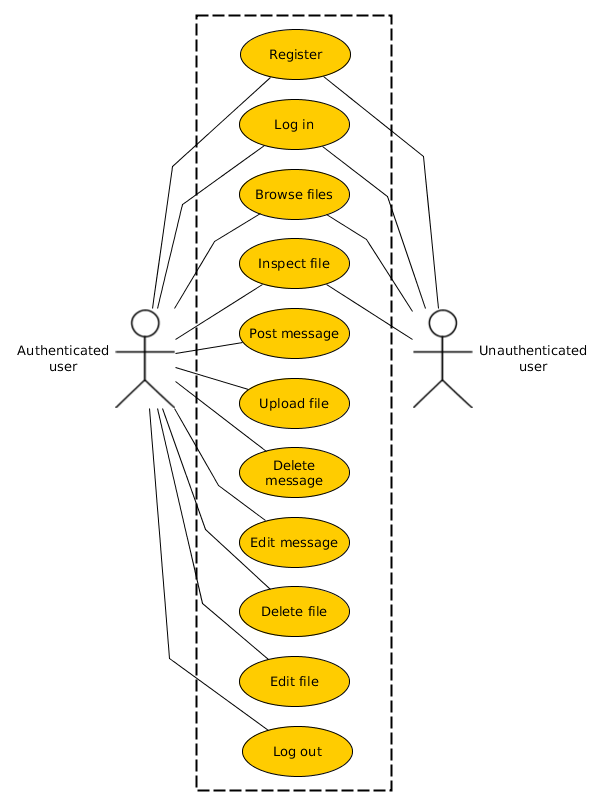
\includegraphics[scale=0.5]{diagrams/use_case.png}
\subsection{User classes}
\paragraph{Unauthenticated user}
Anyone on the web.

\paragraph{Authenticated user}
Someone who has created an account on the server and is currently logged in on that account.

\subsection{Use cases by user class}
\subsubsection{Unauthenticated user}
Unauthenticated users can do the following:
\paragraph{Browse files}
The user lists either all files on the server, or some subset of them by using the search function.
\paragraph{Inspect file / browse messages}
The user selects one file and is shown detailed information about it, in addition to any comments posted on that file.
\paragraph{Upload file}
The user uploads a file to the server.
\paragraph{Post message}
The user posts a message related to some file on the server.

\paragraph{Register}
The user creates an account on the service.
\paragraph{Log in}
The user logs in to an existing account on the server.


\subsubsection{Authenticated user}
Authenticated users can do everything unauthenticated users can. In addition authenticated users can do the following:
\paragraph{Edit file}
The user edits some of the metadata related to a file. It is possible to edit the file's name, description and tags. Other metadata or the file itself are not editable. The file must be originally uploaded by the user trying to edit it.
\paragraph{Delete file}
The user deletes a from the server. All messages related to the file are also deleted. The file must be originally uploaded by the user trying to delete it.

\paragraph{Edit message}
The user edits a message. The message must be originally posted by the user trying to edit it.
\paragraph{Delete message}
The user deletes a message from the server. The message must be originally posted by the user trying to delete it.

\paragraph{Log out}
The user logs out from the server and becomes and unauthenticated user.

\section{System data content}
\subsection{Class diagram}
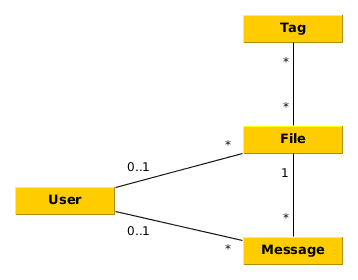
\includegraphics[scale=0.7]{diagrams/class.png}
\subsection{Class attribute details}
\subsubsection{User}
\begin{tabularx}{\textwidth}{|R|R|R|} \hline
\textbf{Attribute} & \textbf{Type} & \textbf{Description}\\ \hline
User name & String & The name of the user account on the server.\\ \hline
Password hash & String & One-way hash of the user's password.\\ \hline
Password salt & String & Additional data that is used in the hashing process to increase security.\\ \hline
\end{tabularx}

\subsubsection{File}
\begin{tabularx}{\textwidth}{|R|R|R|} \hline
\textbf{Attribute} & \textbf{Type} & \textbf{Description}\\ \hline
Uploader & User & The user who uploaded the file to the server.\\ \hline
File name & String & The name of the file\\ \hline
File description & String & Description and context of the file's contents.\\ \hline
Timestamp & Timestamp & The time the file was first uploaded to the server.\\ \hline
File path & String & Path to the file in the server file system.\\ \hline
File size & Integer & The size of the file in bytes.\\ \hline
File type & String & The MIME type of the file, for example text/plain.\\ \hline
\end{tabularx}

\subsubsection{Tag}
\begin{tabularx}{\textwidth}{|R|R|R|} \hline
\textbf{Attribute} & \textbf{Type} & \textbf{Description}\\ \hline
Tag name & String & The name of the tag.\\ \hline
Tag description & String & Additional information and context relating to the tag.\\ \hline
\end{tabularx}

\subsubsection{Message}
\begin{tabularx}{\textwidth}{|R|R|R|} \hline
\textbf{Attribute} & \textbf{Type} & \textbf{Description}\\ \hline
Message poster & User & The user that posted the message.\\ \hline
Related file & File & The file that the message is related to.\\ \hline
Subject & String & The subject of the message.\\ \hline
Body & String & The content of the message.\\ \hline
Timestamp & Timestamp & The time the message was posted on the server.\\ \hline
\end{tabularx}

\section{Database diagram}
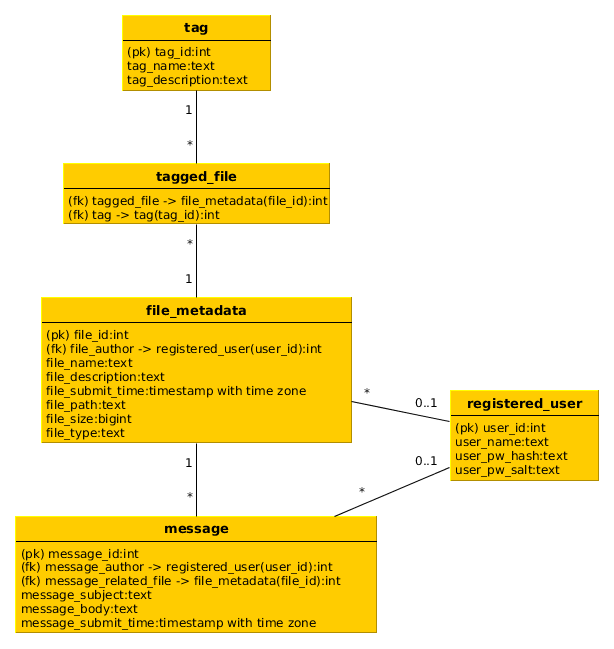
\includegraphics[scale=0.7]{diagrams/database.png}

\section{Application architecture}
The application adheres to the MVC model. Source code is mostly located in the "app" subfolder, with further subfolders for models, views and controllers. Additional libraries are in the folders "lib" and "vendor" in the project root. 

\section{User interface and system components}
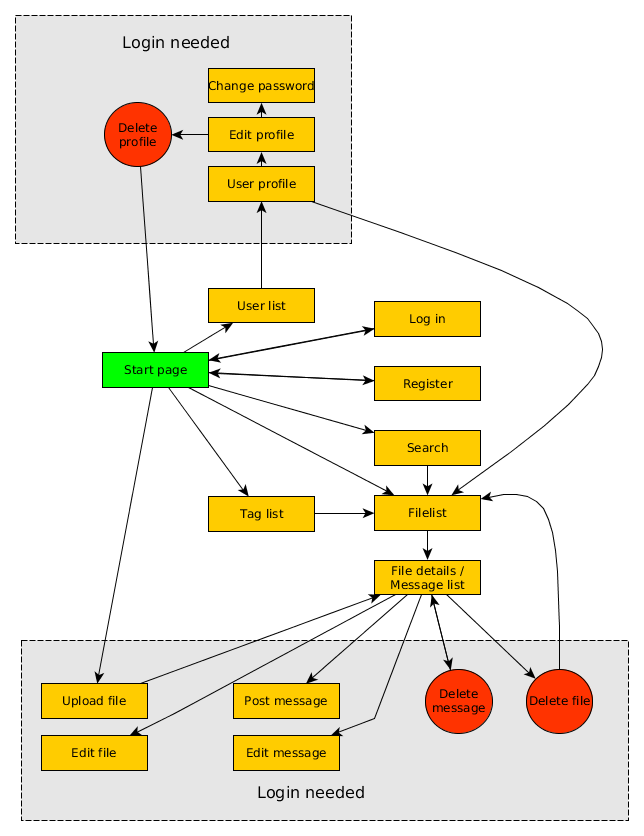
\includegraphics[scale=0.7]{diagrams/pageflow.png}

\section{Instructions for use}


\section{}
\end{document}
